\subsection{YOLOv4-Tiny}

% PLOT input_sizes:
% iou_thresh = 0.3
% score_thresh = 0.25
% default = DIoU-NMS
%            | 448, 480, 512, 544, 576, 608, 640, 672, 704, 736, 768, 800
% default    | 84.121 | 88.215 | 90.856 |
% DIoU-TTA   |
% WBF        |
% WBF-TTA    |

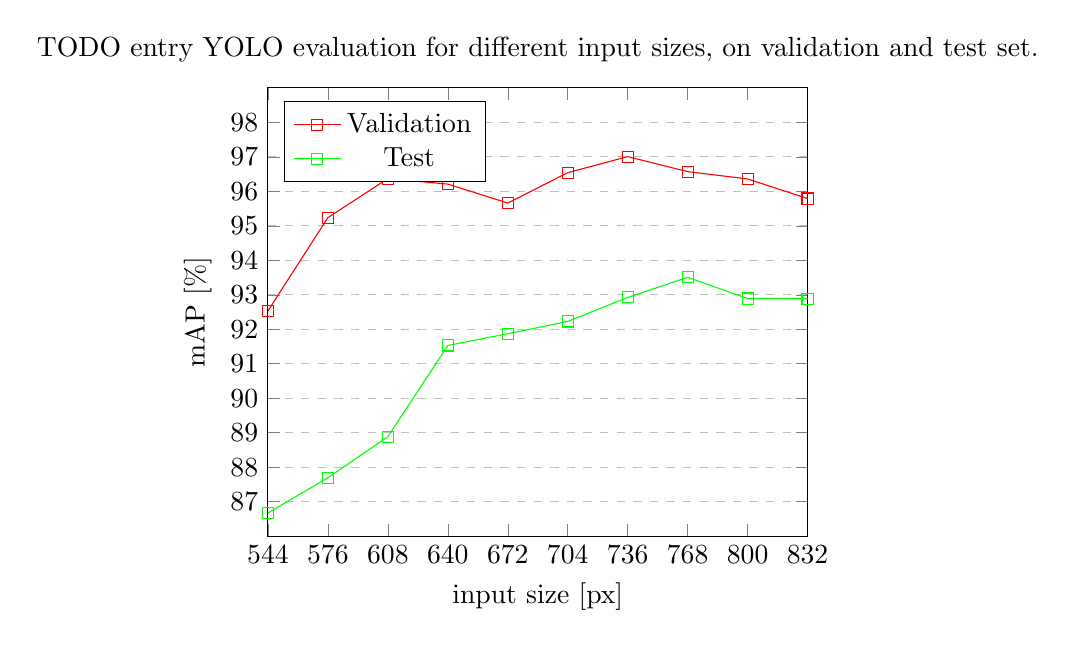
\begin{tikzpicture}
\begin{axis}[
    title={TODO entry YOLO evaluation for different input sizes, on validation and test set.},
    xlabel={input size [px]},
    ylabel={mAP [\%]},
    xmin=544, xmax=832,
    ymin=86, ymax=99,
    xtick={544,576,608,640,672,704,736,768,800,832},
    ytick={87,88,89,90,91,92,93,94,95,96,97,98},
    legend pos=north west,
    ymajorgrids=true,
    grid style=dashed,
]

\addplot[
    color=red,
    mark=square,
]
coordinates {
    % (416,80.289)(448,84.121)(480,88.215)(512,90.856)
    (544,92.534)(576,95.237)(608,96.370)(640,96.210)(672,95.659)(704,96.541)(736,97.006)(768,96.571)(800,96.359)(832,95.791)
};
\addlegendentry{Validation}

\addplot[
    color=green,
    mark=square,
]
coordinates {
    % (416,75.736)(448,79.124)(480,82.634)(512,83.450)
    (544,86.674)(576,87.695)(608,88.884)(640,91.531)(672,91.871)(704,92.227)(736,92.925)(768,93.506)(800,92.890)(832,92.885)
};
\addlegendentry{Test}

\end{axis}
\end{tikzpicture}

\begin{tikzpicture}
\begin{axis}[
    title={TODO entry YOLO evaluation for different input sizes, on validation and test set.},
    xlabel={input size [px]},
    ylabel={mAP [\%]},
    xmin=544, xmax=832,
    ymin=86, ymax=99,
    xtick={544,576,608,640,672,704,736,768,800,832},
    ytick={87,88,89,90,91,92,93,94,95,96,97,98},
    legend pos=north west,
    ymajorgrids=true,
    grid style=dashed,
]

\addplot[
    color=red,
    mark=square,
]
coordinates {
    % (416,80.289)(448,84.121)(480,88.215)(512,90.856)
    (544,92.534)(576,95.237)(608,96.370)(640,96.210)(672,95.659)(704,96.541)(736,97.006)(768,96.571)(800,96.359)(832,95.791)
};
\addlegendentry{Validation}

\addplot[
    color=,
    mark=square,
]
coordinates {
    (416,75.736)(448,79.124)(480,82.634)(512,83.450)
    (544,86.674)(576,87.695)(608,88.884)(640,91.531)(672,91.871)(704,92.227)(736,92.925)(768,93.506)(800,92.890)(832,92.885)
};
\addlegendentry{Test}

\end{axis}
\end{tikzpicture}


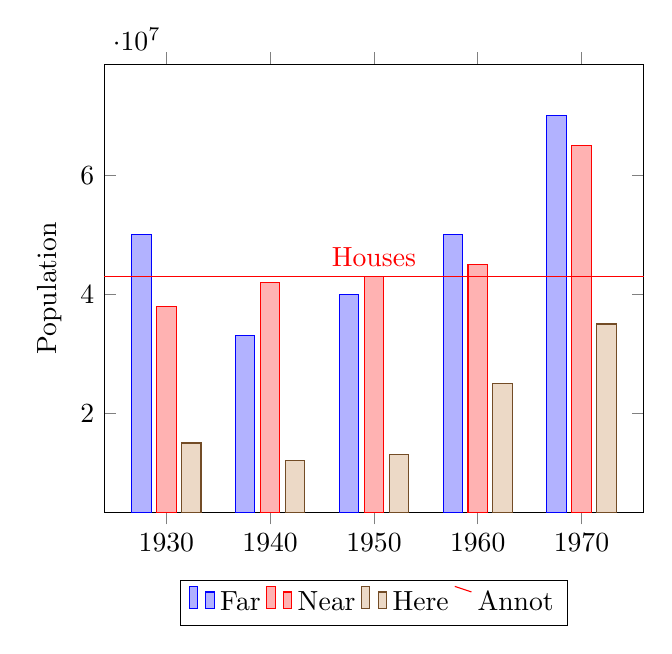
\begin{tikzpicture}
\begin{axis}[
	x tick label style={
		/pgf/number format/1000 sep=},
	ylabel=Population,
	enlargelimits=0.15,
	legend style={at={(0.5,-0.15)},
		anchor=north,legend columns=-1},
	ybar,
	bar width=7pt,
]
\addplot
	coordinates {(1930,50e6) (1940,33e6) (1950,40e6) (1960,50e6) (1970,70e6)};
\addplot
	coordinates {(1930,38e6) (1940,42e6) (1950,43e6) (1960,45e6) (1970,65e6)};
\addplot
	coordinates {(1930,15e6) (1940,12e6) (1950,13e6) (1960,25e6) (1970,35e6)};

\addplot[red,sharp plot,update limits=false]
	coordinates {(1910,4.3e7) (1990,4.3e7)}
	node[above] at (axis cs:1950,4.3e7) {Houses};

\legend{Far,Near,Here,Annot}
\end{axis}
\end{tikzpicture}

\subsubsection{MobileNetV2-UNet}
